\documentclass{article}[10pt]
\usepackage{multicol, enumerate, enumitem, hyperref, color, soul, setspace, parskip, fancyhdr, amssymb, amsthm, amsmath, bbm, latexsym, units, mathtools}
\everymath{\displaystyle}
\usepackage[headsep=0.5cm,headheight=0cm, left=1 in,right= 1 in,top= 1 in,bottom= 1 in]{geometry}

\begin{document}
This is the Answer Key for Module 7 Version C.

31. Determine the domain of the function below.
$$ \frac{6}{25 x^2 + 55 x + 30} $$ 
The solution is $ \text{All Real numbers except } x = a \text{ and } x = b, \text{ where } a \in [-1.63, -1.18] \text{ and } b \in [-1.11, -0.83] $ 

\begin{enumerate}[label=\Alph*.] 
\item $ \text{All Real numbers except } x = a \text{ and } x = b, \text{ where } a \in [-1.63, -1.18] \text{ and } b \in [-1.11, -0.83] $ 

 This is the correct option! 
\item $ \text{All Real numbers.} $ 

 This corresponds to thinking the denominator has complex roots or that rational functions have a domain of all Real numbers. 
\item $ \text{All Real numbers except } x = a, \text{ where } a \in [-1.63, -1.18] $ 

 This corresponds to removing only 1 value from the denominator. 
\item $ \text{All Real numbers except } x = a \text{ and } x = b, \text{ where } a \in [-30.09, -29.89] \text{ and } b \in [-25.05, -24.94] $ 

 This corresponds to not factoring the denominator correctly. 
\item $ \text{All Real numbers except } x = a, \text{ where } a \in [-30.09, -29.89] $ 

 This corresponds to removing a distractor value from the denominator. 
\end{enumerate} 
 
General Comments: The new domain is the intersection of the previous domains.

-----------------------------------------------

32. Solve the rational equation below. Then, choose the interval(s) that the solution(s) belongs to.
$$ \frac{6}{7*x + 9} - -4 = \frac{6}{-56*x - 72} $$ 
The solution is $ -1.52678571429 $ 

\begin{enumerate}[label=\Alph*.] 
\item $ x \in [-2.06,-1.39] $ 

  
\item $ \text{All solutions lead to invalid or complex values in the equation.} $ 

  
\item $ x_1 \in [0.5, 1.26] \text{ and } x_2 \in [-4,0] $ 

  
\item $ x_1 \in [-1.31, -0.83] \text{ and } x_2 \in [-4,0] $ 

  
\item $ x \in [0.5,1.26] $ 

  
\end{enumerate} 
 
General Comments: Distractors are different based on the number of solutions. Remember that after solving, we need to make sure our solution does not make the original equation divide by zero!

-----------------------------------------------

33. Solve the rational equation below. Then, choose the interval(s) that the solution(s) belongs to.
$$ 6*x/(2*x + 2) - 6*x**2/(10*x**2 + 6*x - 4) = 6/(5*x - 2) $$ 
The solution is $ [1/2 + sqrt(3)/2, -sqrt(3)/2 + 1/2] $ 

\begin{enumerate}[label=\Alph*.] 
\item $ x \in [-0.66,-0.25] $ 

  
\item $ x_1 \in [1.18, 2.6] \text{ and } x_2 \in [-1.3,-0.9] $ 

  
\item $ x \in [-0.06,0.7] $ 

  
\item $ x_1 \in [1.18, 2.6] \text{ and } x_2 \in [-0.7,0.3] $ 

  
\item $ \text{All solutions lead to invalid or complex values in the equation.} $ 

  
\end{enumerate} 
 
General Comments: Distractors are different based on the number of solutions. Remember that after solving, we need to make sure our solution does not make the original equation divide by zero!

-----------------------------------------------

34. Choose the equation of the function graphed below.
$$ \text{Graph of the function } f(x) = \frac{-1}{x - 3} + 2 $$ 
\begin{center}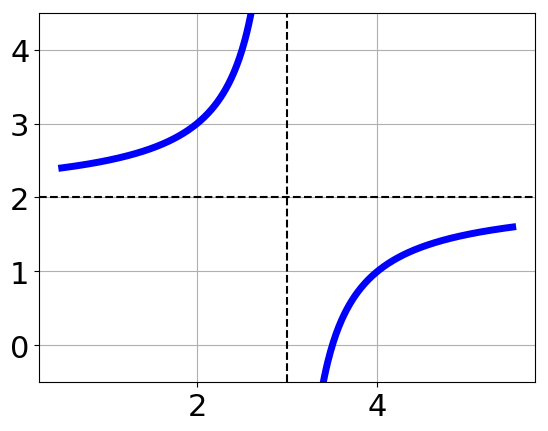
\includegraphics[scale=0.5]{../Figures/question34C.png}\end{center}The solution is $ \frac{-1}{x - 3} + 2 $ 

\begin{enumerate}[label=\Alph*.] 
\item $ \frac{1}{x + 3} + 2 $ 

 Corresponds to using the general form $f(x) = \frac{a}{x+h}+k$ and the opposite leading coefficient. 
\item $ \frac{-1}{x - 3} + 2 $ 

 This is the correct option. 
\item $ \frac{1}{(x + 3)^2} + 2 $ 

 Corresponds to thinking the graph was a shifted version of $\frac{1}{x^2}$, using the general form $f(x) = \frac{a}{x+h}+k$, and the opposite leading coefficient. 
\item $ \frac{-1}{(x - 3)^2} + 2 $ 

 Corresponds to thinking the graph was a shifted version of $\frac{1}{x^2}$. 
\end{enumerate} 
 
General Comments: Remember that the general form of a basic rational equation is $ f(x) = \frac{a}{(x-h)^n} + k$, where $a$ is the leading coefficient (and in this case, we assume is either $1$ or $-1$), $n$ is the degree (in this case, either $1$ or $2$), and $(h, k)$ is the intersection of the asymptotes.

-----------------------------------------------

35. Choose the graph of the equation below.
$$ \frac{-1}{(x - 3)^2} - 3 $$ 
The solution is  
\begin{center}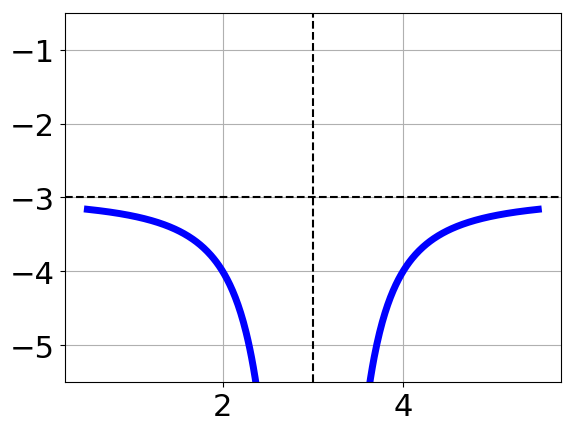
\includegraphics[scale=0.5]{../Figures/question35CD.png}\end{center}\begin{enumerate}[label=\Alph*.] 
\item  
\begin{center}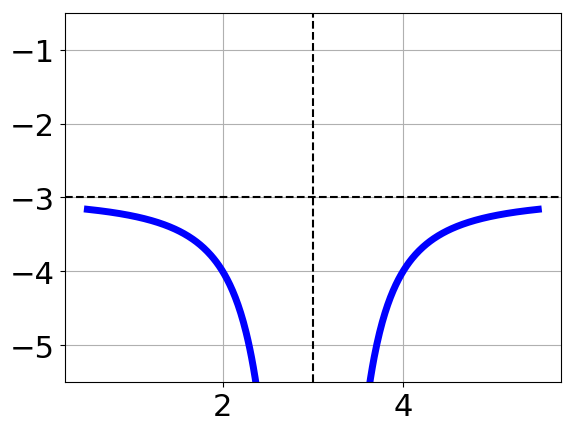
\includegraphics[scale=0.5]{../Figures/question35CD.png}\end{center} 
 
\item  
\begin{center}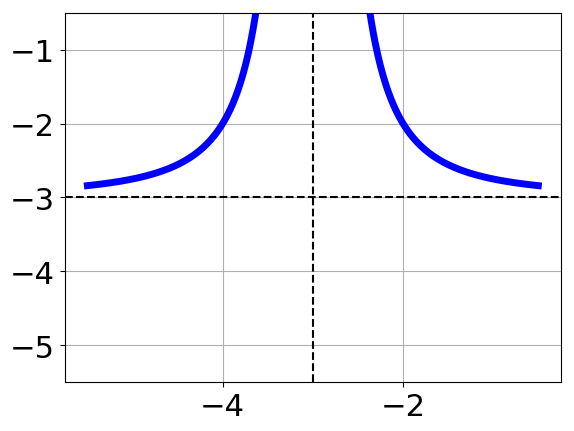
\includegraphics[scale=0.5]{../Figures/question35CC.png}\end{center} 
 
\item  
\begin{center}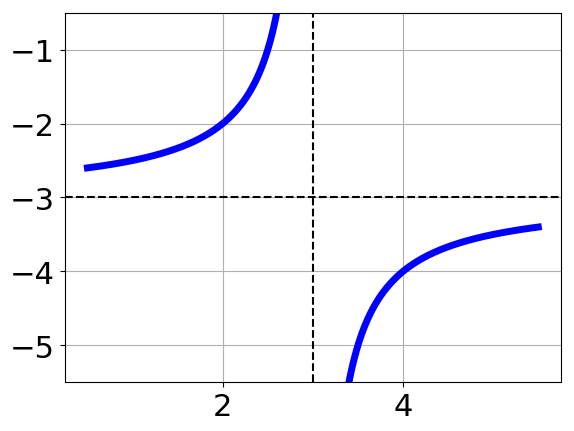
\includegraphics[scale=0.5]{../Figures/question35CA.png}\end{center} 
 
\item  
\begin{center}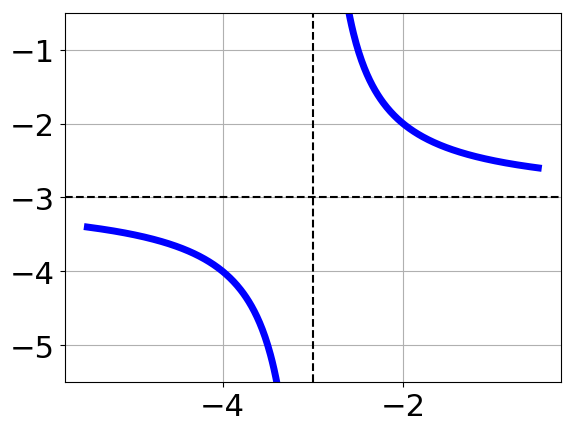
\includegraphics[scale=0.5]{../Figures/question35CB.png}\end{center} 
 
\end{enumerate} 
 
General Comments: Remember that the general form of a basic rational equation is $ f(x) = \frac{a}{(x-h)^n} + k$, where $a$ is the leading coefficient (and in this case, we assume is either $1$ or $-1$), $n$ is the degree (in this case, either $1$ or $2$), and $(h, k)$ is the intersection of the asymptotes.

-----------------------------------------------


\end{document}
